%% 
%% Copyright 2019-2024 Elsevier Ltd
%% 
%% Version 2.4
%% 
%% This file is part of the 'CAS Bundle'.
%% --------------------------------------
%% 
%% It may be distributed under the conditions of the LaTeX Project Public
%% License, either version 1.2 of this license or (at your option) any
%% later version.  The latest version of this license is in
%%    http://www.latex-project.org/lppl.txt
%% and version 1.2 or later is part of all distributions of LaTeX
%% version 1999/12/01 or later.
%% 
%% The list of all files belonging to the 'CAS Bundle' is
%% given in the file `manifest.txt'.
%% 
%% Template article for cas-sc documentclass for 
%% single column output.

%\documentclass[a4paper,fleqn,longmktitle]{cas-sc}
\documentclass[a4paper,fleqn]{cas-sc}

%\usepackage[numbers]{natbib}
%\usepackage[authoryear]{natbib}
\usepackage[authoryear,longnamesfirst]{natbib}

\usepackage{float}
\usepackage{subcaption}
\usepackage{caption}
\usepackage[table]{xcolor}
\usepackage{graphicx}

%%%Author macros
\def\tsc#1{\csdef{#1}{\textsc{\lowercase{#1}}\xspace}}
\tsc{WGM}
\tsc{QE}
\tsc{EP}
\tsc{PMS}
\tsc{BEC}
\tsc{DE}
%%%
%comentario teste para ver o git
\begin{document}
\let\WriteBookmarks\relax
\def\floatpagepagefraction{1}
\def\textpagefraction{.001}
\shorttitle{Neural TCP}
\shortauthors{J.K. Krishnan et~al.}
%\begin{frontmatter}

\title [mode = title]{This is a specimen $a_b$ title}                      
\tnotemark[1,2]

\tnotetext[1]{This document is the results of the research
   project funded by the National Science Foundation.}

\tnotetext[2]{The second title footnote which is a longer text matter
   to fill through the whole text width and overflow into
   another line in the footnotes area of the first page.}


\author[1,3]{J.K. Krishnan}[type=editor,
                        auid=000,bioid=1,
                        prefix=Sir,
                        role=Researcher,
                        orcid=0000-0001-0000-0000]
\cormark[1]
\fnmark[1]
\ead{jkk@example.in}
\ead[url]{www.jkkrishnan.in}

\credit{Conceptualization of this study, Methodology, Software}

\affiliation[1]{organization={Department of Physics, J.K. Institute of Science},
                addressline={Jawahar Nagar}, 
                city={Trivandrum},
%               citysep={}, % Uncomment if no comma needed between city and postcode
                postcode={695013}, 
                state={Kerala},
                country={India}}

\author[2,4]{Han Thane}[style=chinese]

\author[2,3]{William {J. Hansen}}[%
   role=Co-ordinator,
   suffix=Jr,
   ]
\fnmark[2]
\ead{wjh@example.org}
\ead[URL]{https://www.university.org}

\credit{Data curation, Writing - Original draft preparation}

\affiliation[2]{organization={World Scientific University},
                addressline={Street 29}, 
                postcode={1011 NX}, 
                postcodesep={}, 
                city={Amsterdam},
                country={The Netherlands}}

\author[1,3]{T. Rafeeq}
\cormark[2]
\fnmark[1,3]
\ead{t.rafeeq@example.in}
\ead[URL]{www.campus.in}

\affiliation[3]{organization={University of Intelligent Studies},
                addressline={Street 15}, 
                city={Jabaldesh},
                postcode={825001}, 
                state={Orissa}, 
                country={India}}

\cortext[cor1]{Corresponding author}
\cortext[cor2]{Principal corresponding author}
\fntext[fn1]{This is the first author footnote, but is common to third
  author as well.}
\fntext[fn2]{Another author footnote, this is a very long footnote and
  it should be a really long footnote. But this footnote is not yet
  sufficiently long enough to make two lines of footnote text.}

\nonumnote{This note has no numbers. In this work we demonstrate $a_b$
  the formation Y\_1 of a new type of polariton on the interface
  between a cuprous oxide slab and a polystyrene micro-sphere placed
  on the slab.
  }

\begin{abstract}
The advancement and ubiquity of digital networks have fundamentally transformed numerous spheres of human activity. At the heart of this phenomenon, lies the Transmission Control Protocol (TCP) model, whose influence is particularly notable in the exponential growth of the Internet due to its ability to transmit flexibly to any device, through its advanced Congestion Control (CC). Seeking an even more efficient CC mechanism, this work proposes the construction of deep learning neural networks (MLP, LSTM, and CNN) for classifying the level of network congestion. The results attest to models capable of distinguishing, with over 90\% accuracy, between moments of high and low degrees of congestion. With this, it becomes possible to differentiate between congestion and random losses, potentially increasing throughput by up to five times in environments with random losses when combined with CC algorithms.

\noindent\texttt{\textbackslash begin{abstract}} \dots 
\texttt{\textbackslash end{abstract}} and
\verb+\begin{keyword}+ \verb+...+ \verb+\end{keyword}+ 
which
contain the abstract and keywords respectively. 
Each keyword shall be separated by a \verb+\sep+ command.
\end{abstract}

\begin{graphicalabstract}

\includegraphics{figs/cas-grabs.pdf}
\end{graphicalabstract}

\begin{highlights}
\item Research highlights item 1
\item Research highlights item 2
\item Research highlights item 3
\end{highlights}

\begin{keywords}
quadrupole exciton \sep polariton \sep \WGM \sep \BEC
\end{keywords}


\maketitle


\section{Introduction}
%grammarlyGJ%
Digital networks, fundamental to the daily lives of modern society, are widely governed by the TCP transport layer. This predominance derives from the broad range of services available on the internet, accessible through a variety of terminals with different architectures. The internet, which has quickly become accessible to around 95\% of the global population \cite{b0000049}, operates on a set of rules established by the TCP protocol. Such rules, embedded in operating systems, facilitate the application's data exchange through a series of layered structured services, known collectively as the TCP/IP protocol stack.

%grammarly GJ%
A critical element of this stack is the Transport Layer, carried out by Congestion Control (CC). CC is essential to TCP transmissions, adjusting how much data it should transfer in each transmission cycle. A crucial part of CC is the estimation of network congestion level, which, in most available implementations, is performed through losses that have already occurred or variations in delay during data exchange.

%grammarly GJ%
In this context, Deep Learning Networks, such as Multilayer Perceptron (MLP) \cite{b0000062}, Long Short-Term Memory (LSTM) \cite{b0000060}, or Convolutional Neural Network (CNN)  \cite{b0000061} emerge as architectures with promising methods for accurately estimating the level of congestion, before infrastructure saturation.

\subsection{Research questions}
Given the above, this work investigates the performance of these AI architectures, directly used in CC, seeking to answer the following research questions (RQ):


\begin{itemize}
	\item \textbf{QP1: (Congestion Learning by Neural Networks)} Investigate the ability of a neural network to learn to classify the degree of congestion in a network connection, based on the occupancy of an output \textit{buffer} in a topology \textit{dumbell}, present in most Internet connections. 
	\begin{itemize}
		\item \textbf{QP1.1: (Tolerance to Variation in the Number of Flows)} Evaluate whether the learning model is capable of maintaining its accuracy and effectiveness even when there are significant variations in the volume of traffic (flow) on the network.
		\item \textbf{QP1.2: (Applicability to Various CC Mechanisms)} Determine whether the learned model can be effectively applied to flows that are controlled by different types of CC mechanisms. 
	\end{itemize}
	\item \textbf{QP2: (Identification of the Optimal Dimension for Congestion Classifiers)} Define the ideal combination of measures (such as data components and dimensions) to develop congestion classifiers that are both efficient and accurate.
	\item \textbf{QP3: (Gains from Learning in Random Loss Scenarios)} Examine whether a model developed from a neural network, trained with low-dimensional vectors, can lead to better use of available bandwidth, especially in scenarios characterized by random packet losses.
\end{itemize}

Based on the research questions outlined, we carried out a broad study through package-level simulations using ns-3 \cite{b0000058}. The flexibility of ns-3 allows you to explore different versions of TCP, machine learning models and number of flows (up to 40). The simulation results revealed effective performance of neural networks in detecting congestion levels.

This effectiveness also served to apply these models in a practical case: the distinction between random packet losses, a common phenomenon in wireless networks, including Wi-Fi connections and 4G and 5G cellular networks, showing the usefulness of the mechanism with significant improvement in transmission performance in these challenging conditions. To validate our results, we resorted to the use of a specific analytical equation for CC in loss scenarios, proving that the performance of competing protocols is negatively affected in the simulation, according to the literature.

\section{Data Mining}
To build a training dataset, we implemented a ns3  Traffic Analyzer (AT). The AT performs several simulations of a \textit{dumbbell} topology (Figure \ref{fig:dumbell}), a common configuration in network research, which has a central bottleneck and several independent access links. The channels of the stations connected to Router 01 have 2ms delay. In all others, this time is 10ms. The transmission rate is 1Gbs on all channels, with the exception of the one between routers, the bottleneck, which is set to 10, 100, 500 and 1000 Mbps, according to the interested scenarios.

\begin{figure}[!htb]
	\centering
	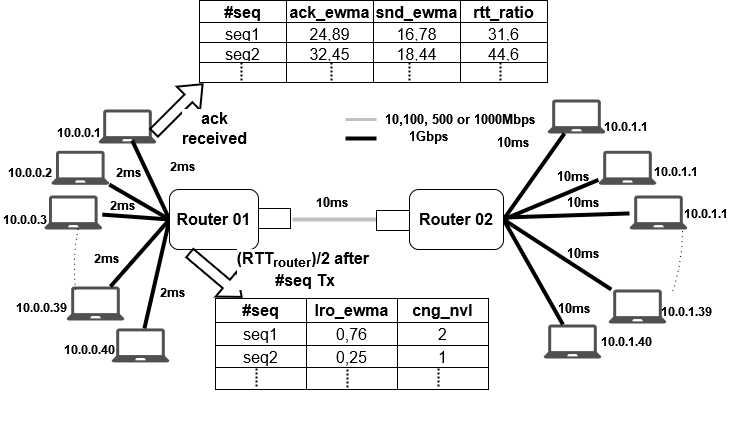
\includegraphics[width=.4\textwidth]{figs//dumbell_final_EN.png}
	\caption{Topology used to acquire training, validation and tests data and for CC mechanisms evaluation..}
	\label{fig:dumbell}
\end{figure}


Through the dumbbell topology, distributed TCP connections are established. Applications are on terminals connected to Router 01 and TCP servers are on those connected to Router 02. Router 01 10.0.0.2 Terminal connects to terminal 10.1.0.2 of Router 02. Likewise, terminal 10.0.2.2 with the 10.1.2.2; 10.0.3.2 with 10.1.3.2 and so on, until - in case of 80 connections - the last connection, between stations 10.0.79.2 and 10.1.79.2. 

The beginning of the connections are spaced of 0.5s to avoid synchronization. Terminal applications were configured to schedule data sending whenever there is space in the \textit{socket} transmission queue. Once such space was identified, each application waits a random time interval $t$, $0\leq t < 70$ to exhaust that queue again. This interval was chosen to maintain flows intensity and, at the same time, to make the simulations more realistic in terms of data send randomness.

The training data, for each bottleneck datarate, came from  60 Vegas TCP P2P flow, established on independent links, transporting data capable of saturating the bottleneck, during a 1.5-minute ns-3 simulations \footnote{For 10Mbps bottleneck, we execute 11 simulations  to take sufficient low congestion data.}. The AT generate two ``.csv'' files per flow. In the first, the following parameters, inspired by Remmy, are recorded for every ACK received by the sender:  
\begin{itemize}
	\item \#seq: Sequence number, present in the ACK packet.
	\item $ack\_ewma$: Weighted exponential moving average of arrival time between ACK packets. 
	\item $snd\_ewma$: Weighted exponential moving average of the interval between the timestamps present in the respective ACK. 
	\item $rtt\_ratio$: Dividing $RTT$ by $RTT_{min}$.
\end{itemize}

To update the second .csv file, whenever a segment is sent in time $t$, the AT schedules an event at $t+RTT_{router}/2$, where $RTT_{router}$ is the expected RTT between the transmitter and the edge router. During the event handling, the learning target parameters are recorded: 
\begin{itemize}
	\item \#seq: Number of seq present in the segment for which the event was scheduled.
	\item $lro\_ewma$: Weighted exponential moving average of the occupation percentage of the \textit{buffer} of the edge router, to which the transmitter is connected (Router 01 in Figure \ref{fig:dumbell}).
	\item $cng\_nvl$: Network congestion level. If $lro\_ewma <= 40\%$, $cng\_nvl=1$ or $cng\_nvl=2$, case $lro\_ewma>=70\%$.
\end{itemize}

All moving averages were calculated in microseconds ($\mu$s), with a weight of 0.8 for new measurements, in order to prioritize the network momentary state. For training accuracy, the analyzer was configured to record when $lro\_ewma <= 40\%$ or $lro\_ewma>=70\%$ only. This design seeks robust models in extreme situations, in case of underutilization or overload.


\section{Data Processing}
\label{sec:dataProcessing}
The data generated by the (AT) goes through the following stages, before forming the input vectors for the neural networks:
\begin{enumerate}
	\item \textit{Inner Join} (IJ): The first step consists of generating a table that associates the  $ack\_ewma$, $snd\_ewma$ and $rtt\_ratio$ measurements, with $lro\_ewma$ and $ cng\_nvl$, through the \#seq columns, present in  both files collected by the AT.
	\item Redundancy Elimination (RE): Lines with identical $ack\_ewma$, $snd\_ewma$ and $rtt\_ratio$ are discarted, keeping the last record throughout the simulation.
	\item Label Balancing (LB): The number of Records with  $cng\_nvl=1$ must be the same as those with  $cng\_nvl=2$. Excess data is disregarded.
	\item Attenuators Cut (AC): Records with $ack\_ewma$, $snd\_ewma$ and $rtt\_ratio$ above the ninetieth percentile ($P_{90}$) are ignored.
	\item Input Normalization (IN): Each of the columns goes through a normalization process, in which its measurements are divided by the maximum value present in it. The normalizers collected from the training data will later be used in all other data that enter the constructed models.
	\end {enumerate}
	The resulting table is used to construct a set $X$, where each element $x_i$ is a vector with components $ack\_ewma$, $snd\_ewma$, $rtt\_ratio$ properly treated. Each $x_i$ receives a class $y_i \in Y=\{0,1\}$, equal to $0$ or $1$, according to the value of $cng\_nvl$. After the mentioned steps, we reached a set $X$ of 20,000 entries, for each training process, executed per bottleneck datarate cenario.


\section{Training Neural Networks - Obtaining the Models}
\subsection{Overview}
%grammarly GJ%
The research attained its objectives using twelve models, varying the ARN (MLP, LSTM, CNN), whose specifications are in Table \ref{tab:especifcacao_redes}, associated with a combination of components ($ack\_ewma$, $snd\_ewma$,$rtt\_ratio$). The type of neural network and the respective input vector components label each model. MLP$_{123}$, for example, refers to the model obtained by the MLP network, receiving the three components as input. LSTM$_{13}$ means model obtained by the LSTM neural network, receiving as input ($ack\_ewma$,$rtt\_ratio$); CNN$_{23}$ to CNN, which receives ($snd\_ewma$,$rtt\_ratio$).

%%%%%%%%%%%%%%%%%%%%%%%%%%%%%%%%%%%%%%%%%%%%%%%%%%%%%%
\begingroup

\begin{table}[!htb]
	\footnotesize
	\caption{Neural networks Configuration }
	\centering
\begin{tabular}{|c|c|c|}
	\hline
\multicolumn{3}{|c|}{epoch:3000; batch size 64; learning rate: 0.0001}\\ \hline

	MLP&LSTM&CNN  \\
	\hline
	
	\begin{minipage} [t] {0.30\textwidth}
		\begin{flushleft}
			-Input: 3 dimensional vectors.\\
			-Layers: 3 (20 RELU).\\
			-Output: Sigmoid.
		\end{flushleft}
	\end{minipage}
	
	& \begin{minipage} [t] {0.30\textwidth}
		\begin{flushleft}
			-Input: Matrix 3x3.\\
			-Layers: 2 (each one with 3 LSTM - $30\%$ \textit{dropout} ).\\
			-Output: Sigmoid. 
		\end{flushleft}
	\end{minipage} 
	& \begin{minipage} [t] {0.33\textwidth}
		\begin{flushleft}
			-Input: Image Vectors 3X3@1.\\
			-Convolution:16 maps - 1x3\\
			-Stride: [1,1] \\
			-Convolution Output: RELU\\
			-Pooling:  \textit{maxpooling}, [1,2]. \\
			-Flattening: 64 RELU inputs.\\ 
			-Output: Sigmoid. \end{flushleft}\end{minipage} \\ \hline
	%\multicolumn{3}{epoch:3000; batch size 64; learnin rate 0.0001}\\ \hline
	\end{tabular}	
	\label{tab:especifcacao_redes}
\end{table}
\endgroup
%%%%%%%%%%%%%%%%%%%%%%%%%%%%%%%%%%%%%%%%%%%%%%%%%%%%%%%%%%

%grammarly GJ%
Accuracy, Error, Precision, Recall, and F1, obtained from the \textit{Receiver operating characteristics} (ROC) analysis \footnote{\url{http://mlwiki.org/index.php /ROC_Analysis\#ROC_Space}}, will be used to compare the models extracted from learning networks. The ROC space is constructed from a Cartesian plane, with the abscissa and ordering associated, respectively, with the rates of false positives, or \textit{False Positive Rate} (FPR), and true positives, or \textit {True Positive Rate} (TPR), for a data set offered to the model.

\subsection{Training Vector Transformations}\label{sec:espec_transf_modelos}

%grammarly GJ%
For each of the ARNs, there was a need to transform the vectors from the set $X$. Transformations description uses three-dimensional vectors, with the components $ack\_ewma$, $snd\_ewma$, and $rtt\_ratio$, as it is analogous to those with one or two components. Regarding MLP, for example, the transformation was direct, without more elaborated rearrangement (Figure \ref{fig:transformacao_mlp}).

\begin{figure}[!htb]
	\centering
	\begin{minipage}{0.32\textwidth}
		{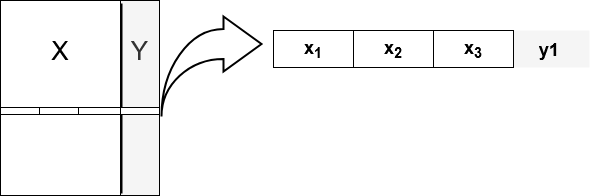
\includegraphics[width=\textwidth]{figs/transformacao_dados_MLP.png}}
		\subcaption{MLP Vectors.}
		\label{fig:transformacao_mlp}
	\end{minipage}
	\hfill
	\begin{minipage}{0.34\textwidth}
		{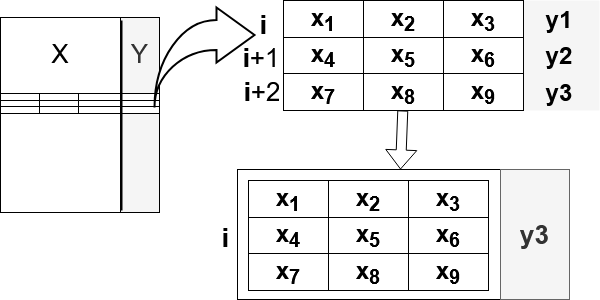
\includegraphics[width=\textwidth]{figs/transformacao_dados_LSTM.png}}
		\subcaption{LSTM Vectors.}
		\label{fig:transformacao_LSTM}
	\end{minipage}
	\hfill
	\begin{minipage}{0.32\textwidth}
		{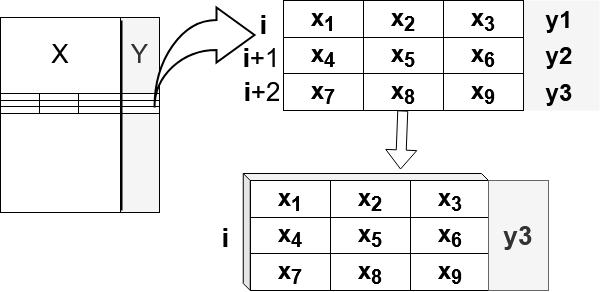
\includegraphics[width=\textwidth]{figs/transformacao_dados_CNN.png}}
		\subcaption{CNN Vectors.}
		\label{fig:transformacao_CNN}
	\end{minipage}
	%\captionsetup{subrefformat=parens}	
	\caption{NNA data transformations.}
	\label{fig:desempenhogeneralizacao}
\end{figure}

%grammGJ
The ARN based on LSTM and CNN required elaborate transformations. In LSTN, considering that $X$ has $m$ elements, each element $x_i$ $(i+2\leq m)$, accompanied by two consecutive vectors, will give rise to an entry in the LSTM network, associated with the class of the third sequence vector (Figure \ref{fig:transformacao_LSTM}). For the CNN architecture, the $X$ vectors were also grouped consecutively by three and later reformatted, forming a kind of ``image'' of 3x3 pixels with one channel.  (Figure \ref{fig:transformacao_CNN}). All training was carried out with 3000 epochs, batch size equal to 64, and a learning rate of 0.0001, using the Keras library from the default configuration of the Google Colab environment. 20\% of the 40,000 entries were reserved for testing, while the rest were for training and validation.

\section{Model Assessment and Selection (QP1)} 

\subsection{Result Analysis - Test Data}\label{sec:analysis_training}
\hfill
\begin{minipage}{0.45\textwidth}
	\begingroup
	\begin{tiny}	
		\setlength{\tabcolsep}{3pt}
		\renewcommand{\arraystretch}{1.15}
		%%%%%%%%%%%%%%%%%%%%%%%%%%%%%%%%%%%%%%
		
		
		\begin{tabular*}{\textwidth}{@{} CCCCCC@{} }
			\toprule
			Modelo&Acurácia&Erro&Precisão&Recall&F1 \\
			\midrule
			MLP$_{123}$ & $0.997$ & $0.003$ & $0.997$ & $0.998$ & $0.997$ \\
			MLP$_{13}$ & $0.998$ & $0.002$ & $1.000$ & $0.995$ & $0.998$ \\
			MLP$_{23}$ & $0.998$ & $0.002$ & $1.000$ & $0.995$ & $0.997$ \\
			MLP$_{12}$ & $0.547$ & $0.453$ & $0.388$ & $0.582$ & $0.465$ \\
			LSTM$_{123}$ & $0.994$ & $0.006$ & $0.986$ & $1.000$ & $0.993$ \\
			LSTM$_{13}$ & $0.994$ & $0.006$ & $0.984$ & $1.000$ & $0.992$ \\
			LSTM$_{23}$ & $0.994$ & $0.006$ & $0.985$ & $1.000$ & $0.992$ \\
			LSTM$_{12}$ & $0.418$ & $0.582$ & $0.661$ & $0.370$ & $0.475$ \\
			CNN$_{123}$ & $0.994$ & $0.006$ & $0.985$ & $0.999$ & $0.992$ \\
			CNN$_{13}$ & $0.981$ & $0.019$ & $0.959$ & $0.994$ & $0.976$ \\
			CNN$_{23}$ & $0.978$ & $0.022$ & $0.950$ & $0.994$ & $0.972$ \\
			CNN$_{12}$ & $0.502$ & $0.498$ & $0.658$ & $0.419$ & $0.512$ \\    		
			\bottomrule
		\end{tabular*}
		\vspace{-0.3cm}
		\captionof{table}{Metrics on 10Mbps bottleneck.}
		\label{tab:metricas_10Mbps_teste}
	\end{tiny}
	\endgroup
\end{minipage}
\hfill
\begin{minipage}{0.45\textwidth}
	\begingroup
	\begin{tiny}	
		\setlength{\tabcolsep}{3pt}
		\renewcommand{\arraystretch}{1.15}
		%%%%%%%%%%%%%%%%%%%%%%%%%%%%%%%%%%%%%%
		
		
		\begin{tabular*}{\textwidth}{@{} CCCCCC@{} }
			\toprule
			Modelo&Acurácia&Erro&Precisão&Recall&F1 \\
			\midrule
				MLP$_{123}$ & $0.998$ & $0.002$ & $0.999$ & $0.996$ & $0.998$ \\
				MLP$_{13}$ & $0.999$ & $0.001$ & $1.000$ & $0.998$ & $0.999$ \\
				MLP$_{23}$ & $0.997$ & $0.003$ & $0.999$ & $0.995$ & $0.997$ \\
				MLP$_{12}$ & $0.571$ & $0.429$ & $0.447$ & $0.589$ & $0.508$ \\
				LSTM$_{123}$ & $0.999$ & $0.001$ & $0.997$ & $1.000$ & $0.998$ \\
				LSTM$_{13}$ & $0.999$ & $0.001$ & $0.998$ & $0.999$ & $0.999$ \\
				LSTM$_{23}$ & $0.999$ & $0.001$ & $0.997$ & $0.999$ & $0.998$ \\
				LSTM$_{12}$ & $0.754$ & $0.246$ & $0.648$ & $0.661$ & $0.654$ \\
				CNN$_{123}$ & $0.998$ & $0.002$ & $0.997$ & $0.998$ & $0.998$ \\
				CNN$_{13}$ & $0.996$ & $0.004$ & $0.998$ & $0.990$ & $0.994$ \\
				CNN$_{23}$ & $0.996$ & $0.004$ & $0.999$ & $0.990$ & $0.995$ \\
				CNN$_{12}$ & $0.746$ & $0.254$ & $0.618$ & $0.655$ & $0.636$ \\    		
			\bottomrule
		\end{tabular*}
		\vspace{-0.3cm}
		\captionof{table}{Metrics on 100Mbps bottleneck.}
		\label{tab:metricas_100Mbps_teste}
	\end{tiny}
	\endgroup
\end{minipage}

\hfill
\begin{minipage}{0.45\textwidth}
	\vspace{0.5cm}
	\begingroup
	\begin{tiny}	
		\setlength{\tabcolsep}{3pt}
		\renewcommand{\arraystretch}{1.15}
		%%%%%%%%%%%%%%%%%%%%%%%%%%%%%%%%%%%%%%
		
		
		\begin{tabular*}{\textwidth}{@{} CCCCCC@{} }
			\toprule
			Modelo&Acurácia&Erro&Precisão&Recall&F1 \\
			\midrule
				MLP$_{123}$ & $0.912$ & $0.088$ & $0.932$ & $0.894$ & $0.913$ \\
				MLP$_{13}$ & $0.902$ & $0.098$ & $0.937$ & $0.876$ & $0.906$ \\
				MLP$_{23}$ & $0.899$ & $0.101$ & $0.911$ & $0.887$ & $0.899$ \\
				MLP$_{12}$ & $0.652$ & $0.348$ & $0.737$ & $0.629$ & $0.679$ \\
				LSTM$_{123}$ & $0.894$ & $0.106$ & $0.857$ & $0.927$ & $0.891$ \\
				LSTM$_{13}$ & $0.909$ & $0.091$ & $0.903$ & $0.916$ & $0.909$ \\
				LSTM$_{23}$ & $0.907$ & $0.093$ & $0.911$ & $0.904$ & $0.908$ \\
				LSTM$_{12}$ & $0.605$ & $0.395$ & $0.392$ & $0.689$ & $0.500$ \\
				CNN$_{123}$ & $0.890$ & $0.110$ & $0.850$ & $0.925$ & $0.886$ \\
				CNN$_{13}$ & $0.906$ & $0.094$ & $0.955$ & $0.870$ & $0.911$ \\
				CNN$_{23}$ & $0.906$ & $0.094$ & $0.954$ & $0.872$ & $0.911$ \\
				CNN$_{12}$ & $0.603$ & $0.397$ & $0.369$ & $0.699$ & $0.483$ \\    		
			\bottomrule
		\end{tabular*}
		\vspace{-0.3cm}
		\captionof{table}{Metrics on 500Mbps bottleneck.}
		\label{tab:metricas_500Mbps_teste}
	\end{tiny}
	\endgroup
\end{minipage}
\hfill
\begin{minipage}{0.45\textwidth}
	\vspace{0.5cm}
	\begingroup
	\begin{tiny}	
		\setlength{\tabcolsep}{3pt}
		\renewcommand{\arraystretch}{1.15}
		%%%%%%%%%%%%%%%%%%%%%%%%%%%%%%%%%%%%%%
		
		
		\begin{tabular*}{\textwidth}{@{} CCCCCC@{} }
			\toprule
			Modelo&Acurácia&Erro&Precisão&Recall&F1 \\
			\midrule
				MLP$_{123}$ & $0.8590$ & $0.1410$ & $0.8690$ & $0.8580$ & $0.8630$ \\
				MLP$_{13}$ & $0.8480$ & $0.1520$ & $0.8650$ & $0.8380$ & $0.8510$ \\
				MLP$_{23}$ & $0.8480$ & $0.1520$ & $0.8520$ & $0.8360$ & $0.8440$ \\
				MLP$_{12}$ & $0.5150$ & $0.4850$ & $0.1700$ & $0.5640$ & $0.2610$ \\
				LSTM$_{123}$ & $0.8290$ & $0.1710$ & $0.7880$ & $0.8700$ & $0.8270$ \\
				LSTM$_{13}$ & $0.8440$ & $0.1560$ & $0.8570$ & $0.8440$ & $0.8510$ \\
				LSTM$_{23}$ & $0.8230$ & $0.1770$ & $0.7910$ & $0.8560$ & $0.8220$ \\
				LSTM$_{12}$ & $0.5100$ & $0.4900$ & $0.4090$ & $0.5340$ & $0.4630$ \\
				CNN$_{123}$ & $0.8470$ & $0.1530$ & $0.8370$ & $0.8630$ & $0.8500$ \\
				CNN$_{13}$ & $0.8420$ & $0.1580$ & $0.8530$ & $0.8430$ & $0.8480$ \\
				CNN$_{23}$ & $0.8410$ & $0.1590$ & $0.8520$ & $0.8420$ & $0.8470$ \\
				CNN$_{12}$ & $0.5220$ & $0.4780$ & $0.4460$ & $0.5470$ & $0.4910$ \\
			\bottomrule
		\end{tabular*}
		\vspace{-0.3cm}
		\captionof{table}{Metrics on 1000Mbps bottleneck.}
		\label{tab:metricas_1000Mbps_teste}
	\end{tiny}
	\endgroup	
\end{minipage}
\\
\\
\\
\begingroup
\captionsetup[figure]{font=tiny}
\hfill
\begin{minipage}{0.25\textwidth}
	\centering
	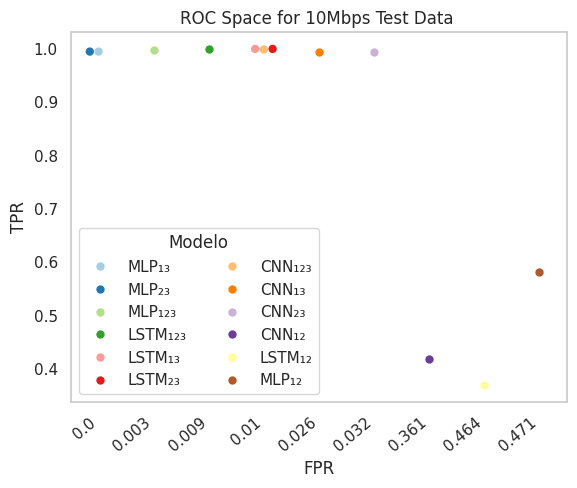
\includegraphics[width=1.0\textwidth]{./figs/ROC-Space-Test-Data-10Mbps.png}
	\captionof{figure}{ROC space test Data 10Mbps.}
	\label{fig:ROCDesempenhoteste10Mbps}	
\end{minipage}
%\hfill
\begin{minipage}{0.25\textwidth}
	\centering
	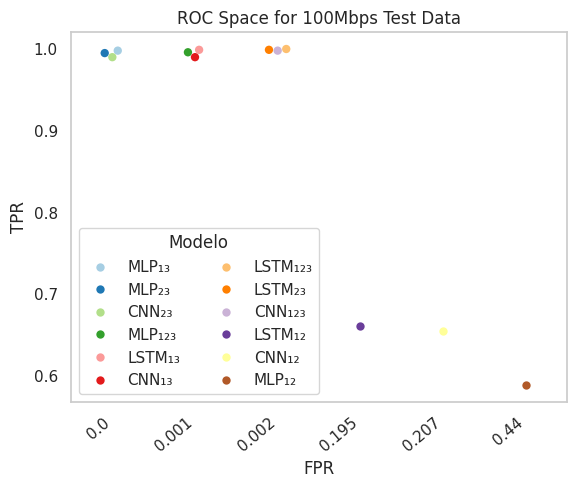
\includegraphics[width=1.0\textwidth]{./figs/ROC-Space-Test-Data-100Mbps.png}
	\captionof{figure}{ROC space test Data 100Mbps.}
	\label{fig:ROCDesempenhoteste100Mbps}	
\end{minipage}
%\hfill
%\\
%\\
%\hfill
\begin{minipage}{0.25\textwidth}
	\centering
	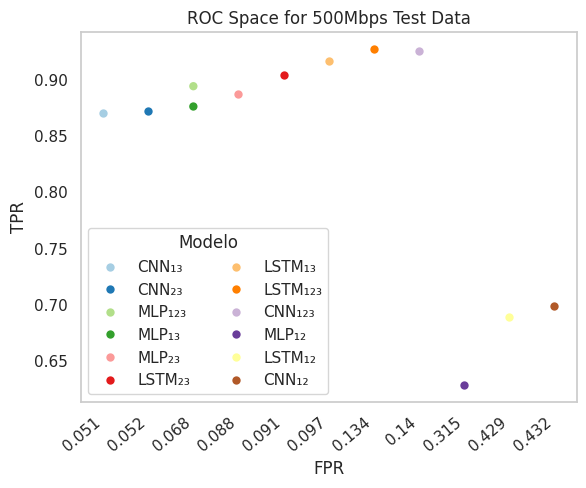
\includegraphics[width=1.0\textwidth]{./figs/ROC-Space-Test-Data-500Mbps.png}
	\captionof{figure}{ROC space test Data 500Mbps.}
	\label{fig:ROCDesempenhoteste500Mbps}	
\end{minipage}
%\hfill
\begin{minipage}{0.25\textwidth}
	\centering
	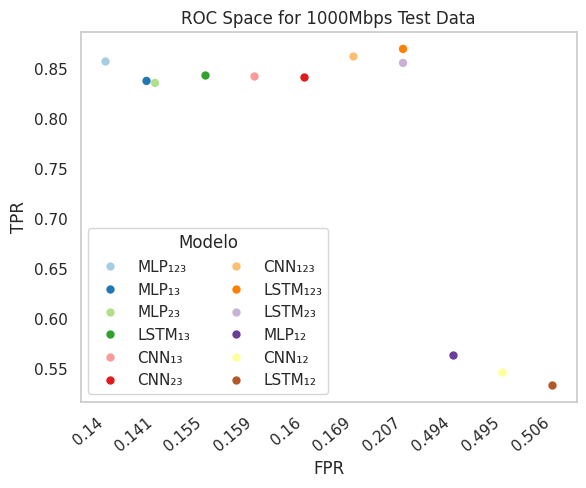
\includegraphics[width=1.0\textwidth]{./figs/ROC-Space-Test-Data-1000Mbps.png}
	\captionof{figure}{ROC space test Data 1000Mbps.}
	\label{fig:ROCDesempenhoteste1000Mbps}	
\end{minipage}
%\hfill
\endgroup



\subsection{Generalization capacity of models (QP1.1, QP1.2, QP 2)}
%GGJ
The models had their generalization capacity measured on data from flows that did not participate in the training. \text To achieve this, new simulations were carried out using the topology in Figure \ref{fig:dumbell}, along the same lines as that carried out to collect the training data; however, using different numbers of stations (and their flows) connected to the bottleneck (5, 10, 20, 40) and  CC algorithm (NewReno, CUBIC, BBR and Vegas). Since TCP-Vegas did not produce occupancy above $70\%$ on the edge router for 05 flows, there were $15$ valid simulations.


After the data preparation processing described previously, each simulation provided a set $X$ of 4000 inputs. Of these 4000 entries, 70\% (2,800) were randomly selected, transformed, and classified by each of the $09$ surviving models (Section \ref{sec:analise_treinamento}). The results, using average values of the metrics, are presented in Table \ref{tab:performancegeneralizacao}:

In general, the models demonstrated excellent generalization capacity. In Table \ref{tab:performancegeneralizacao}, the two values corresponding to the best performance are highlighted in each column, including ties. It can be seen that, again, the MLP$_{23}$, CNN$_{123}$ and CNN$_{13}$ models stand out. Component 3, $rtt\_ratio$ is always present in the best answers.

%GGJ%
The models have an impressive performance, as can be seen in the corresponding ROC space (Figure \ref{fig:performancegeneralizacao2}), collected from the confusion matrix obtained in each round of classification (each color is a variation of CC and number of flows). The density of points around the position (0,1) and the straight line TPR=1 reaffirm the models MLP$_{23}$(Fig.\ref{fig:performancegeneralizacaoMLP23}), CNN$_{123}$(Fig . \ref{fig:performancegeneralizacaoCNN123}) and CNN$_{13}$(Fig. \ref{fig:performancegeneralizacaoCNN13}) as the best performers. The CNN$_{23}$ model (Fig. \ref{fig:performancegeneralizacaoCNN23}) is worth highlighting, with good distribution in the ROC space, however, falling short of the three previously mentioned.



	\begin{figure}
	\centering
	
	\begin{minipage}[t]{0.46\textwidth} % or '[b]', if desired
		\centering
		
		
		%\captionbox[Caption]{Caption\par Source:\label{fig:dummy}}{
			\begin{subfigure}[t]{0.33\textwidth}
				
				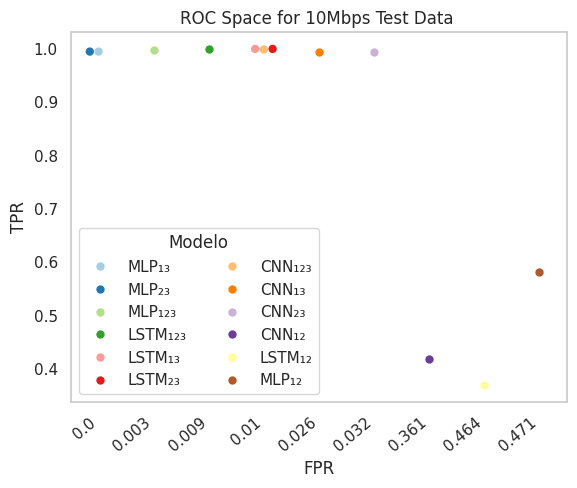
\includegraphics[draft=false, width=\textwidth]{./figs/ROC-Space-Test-Data-10Mbps.png} 
				\caption{Image A}
				\label{fig:1a}
			\end{subfigure}%
			~
			\begin{subfigure}[t]{0.33\textwidth}
				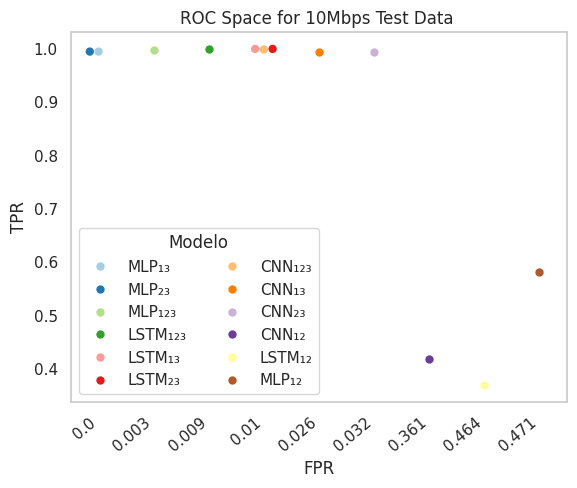
\includegraphics[draft=false, width=\textwidth]{./figs/ROC-Space-Test-Data-10Mbps.png} 
				\caption{Image B}
				\label{fig:2a}
			\end{subfigure}%
			~
			%\medskip % create some vertical separation
			\begin{subfigure}[t]{0.33\textwidth}
				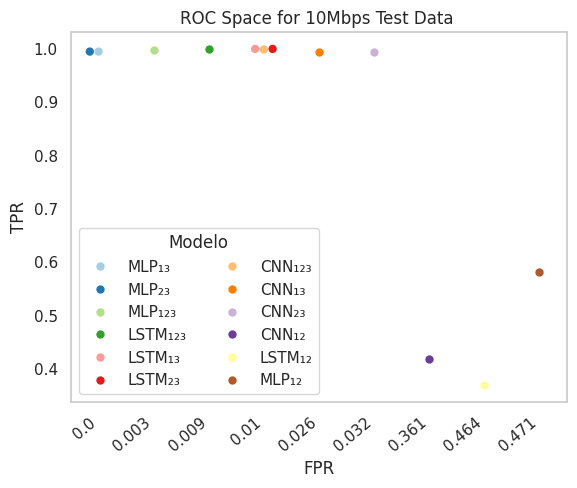
\includegraphics[draft=false, width=\textwidth]{./figs/ROC-Space-Test-Data-10Mbps.png} 
				\caption{Image C}
				\label{fig:1c}
			\end{subfigure}%
			~
			
			\begin{subfigure}[t]{0.33\textwidth}
				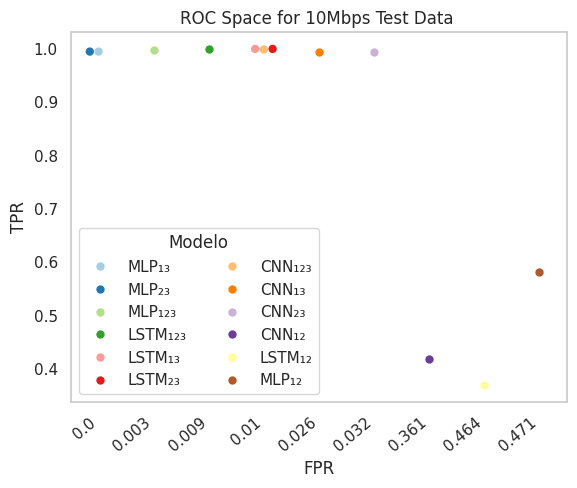
\includegraphics[draft=false, width=\textwidth]{./figs/ROC-Space-Test-Data-10Mbps.png} 
				\caption{Image D}
				\label{fig:1a}
			\end{subfigure}%
			~
			\begin{subfigure}[t]{0.33\textwidth}
				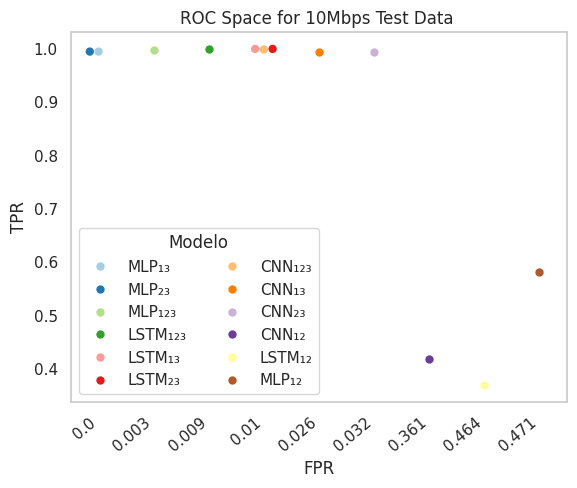
\includegraphics[draft=false, width=\textwidth]{./figs/ROC-Space-Test-Data-10Mbps.png} 
				\caption{Image E}
				\label{fig:2a}
			\end{subfigure}%
			~
			%\medskip % create some vertical separation
			\begin{subfigure}[t]{0.33\textwidth}
				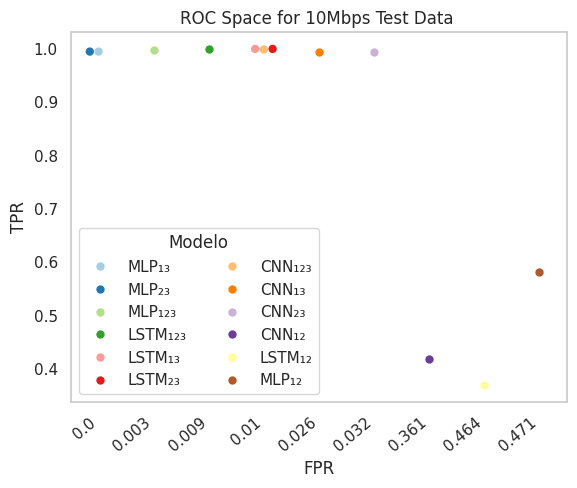
\includegraphics[draft=false, width=\textwidth]{./figs/ROC-Space-Test-Data-10Mbps.png} 
				\caption{Image F}
				\label{fig:1c}
			\end{subfigure}%
			~%Ten que ter uma linha depois do ~
			
			\begin{subfigure}[t]{0.33\textwidth}
				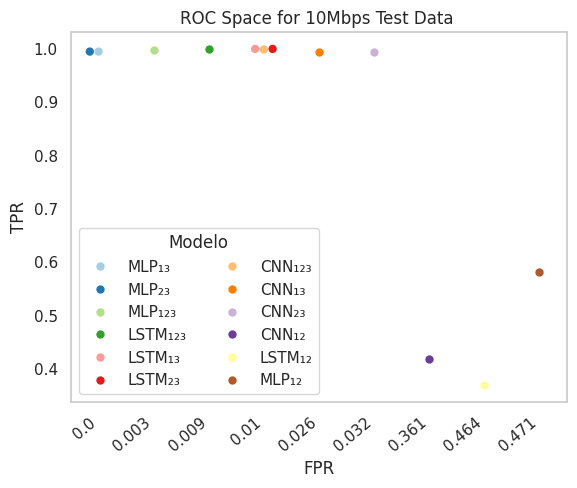
\includegraphics[draft=false, width=\textwidth]{./figs/ROC-Space-Test-Data-10Mbps.png} 
				\caption{Image G}
				\label{fig:1a}
			\end{subfigure}%
			~
			\begin{subfigure}[t]{0.33\textwidth}
				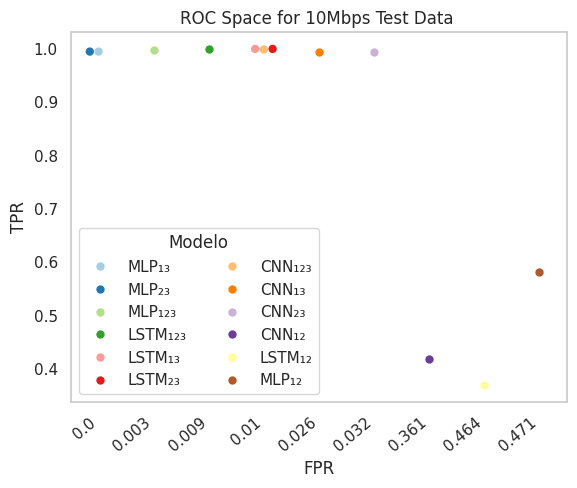
\includegraphics[draft=false, width=\textwidth]{./figs/ROC-Space-Test-Data-10Mbps.png} 
				\caption{Image H}
				\label{fig:2a}
			\end{subfigure}%
			~
			%\medskip % create some vertical separation
			\begin{subfigure}[t]{0.33\textwidth}
				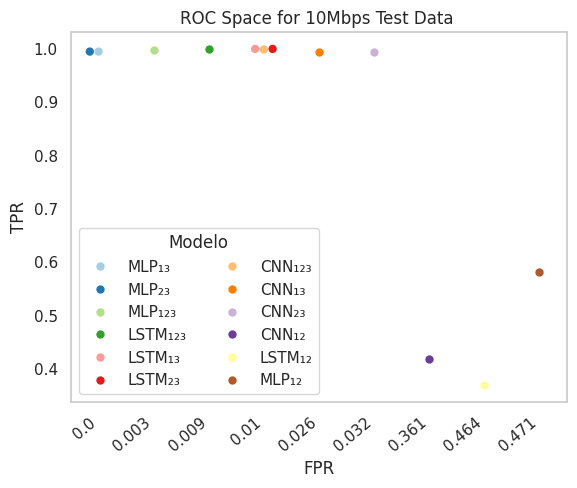
\includegraphics[draft=false, width=\textwidth]{./figs/ROC-Space-Test-Data-10Mbps.png} 
				\caption{Image I}
				\label{fig:1c}
			\end{subfigure}%		
			~
			%}
		\hfill
		\caption{ Image Collection 1\hspace{10cm}}
		\label{fig:Pasnatsch}
		
	\end{minipage}
	\hfill%
	\begin{minipage}[t]{0.46\textwidth} % or '[b]', if desired
		%\captionbox[Caption]{Caption\par Source:\label{fig:dummy}}{
			\begin{subfigure}[t]{0.33\textwidth}
				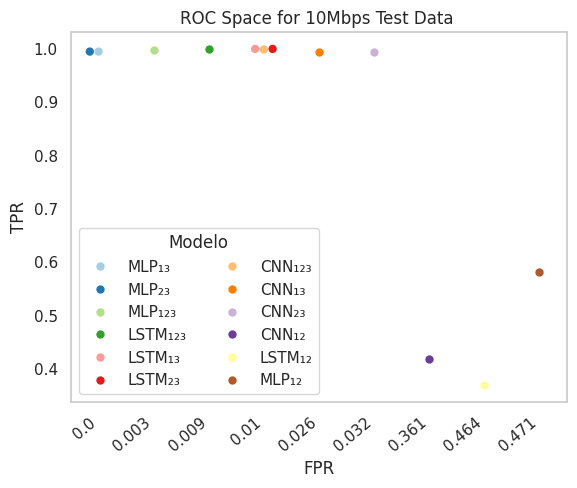
\includegraphics[draft=false, width=\textwidth]{./figs/ROC-Space-Test-Data-10Mbps.png} 
				\caption{Image A}
				\label{fig:1a}
			\end{subfigure}%
			~
			\begin{subfigure}[t]{0.33\textwidth}
				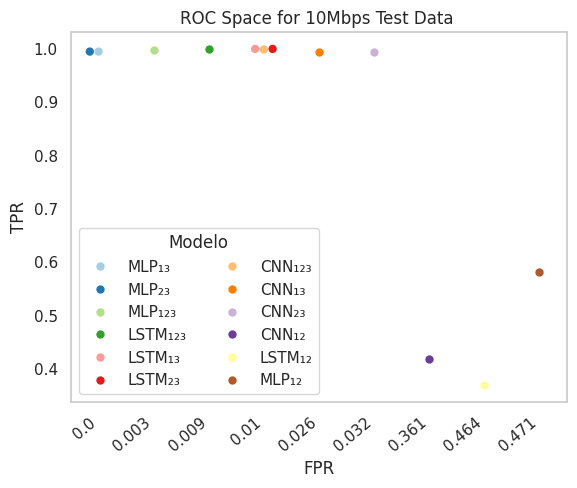
\includegraphics[draft=false, width=\textwidth]{./figs/ROC-Space-Test-Data-10Mbps.png} 
				\caption{Image B}
				\label{fig:2a}
			\end{subfigure}%
			~
			%\medskip % create some vertical separation
			\begin{subfigure}[t]{0.33\textwidth}
				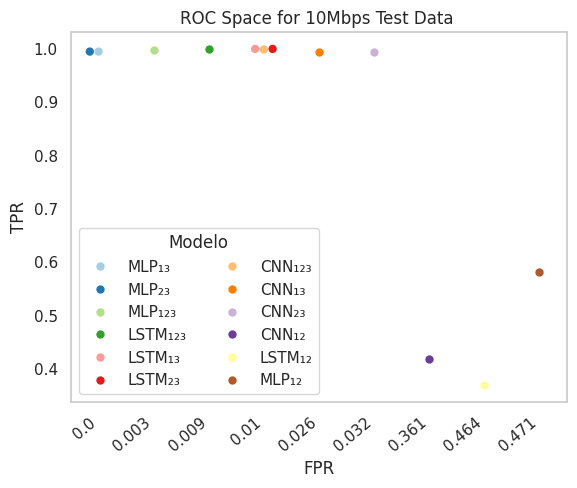
\includegraphics[draft=false, width=\textwidth]{./figs/ROC-Space-Test-Data-10Mbps.png} 
				\caption{Image C}
				\label{fig:1c}
			\end{subfigure}%
			~
			
			\begin{subfigure}[t]{0.33\textwidth}
				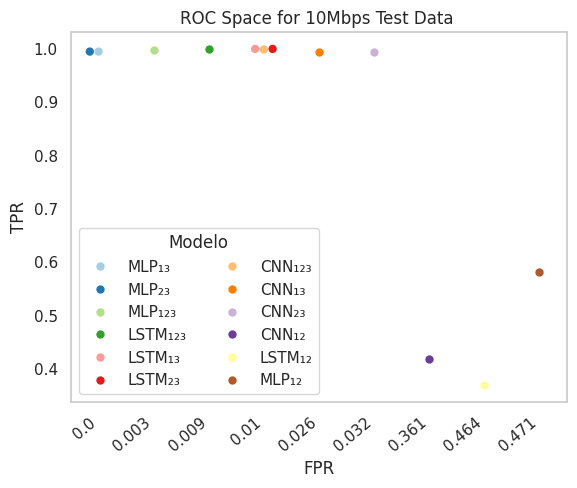
\includegraphics[draft=false, width=\textwidth]{./figs/ROC-Space-Test-Data-10Mbps.png} 
				\caption{Image D}
				\label{fig:1a}
			\end{subfigure}%
			~
			\begin{subfigure}[t]{0.33\textwidth}
				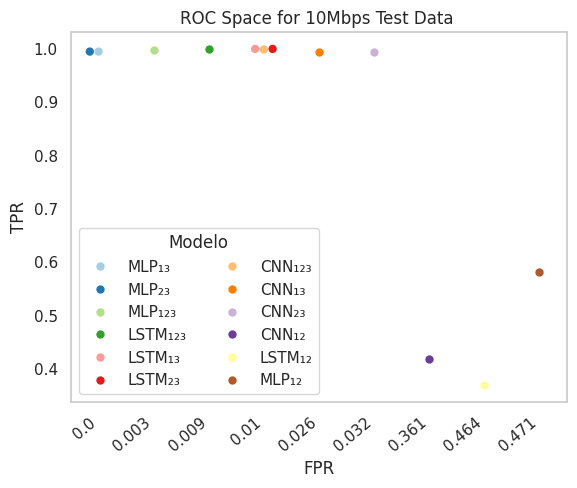
\includegraphics[draft=false, width=\textwidth]{./figs/ROC-Space-Test-Data-10Mbps.png} 
				\caption{Image E}
				\label{fig:2a}
			\end{subfigure}%
			~
			%\medskip % create some vertical separation
			\begin{subfigure}[t]{0.33\textwidth}
				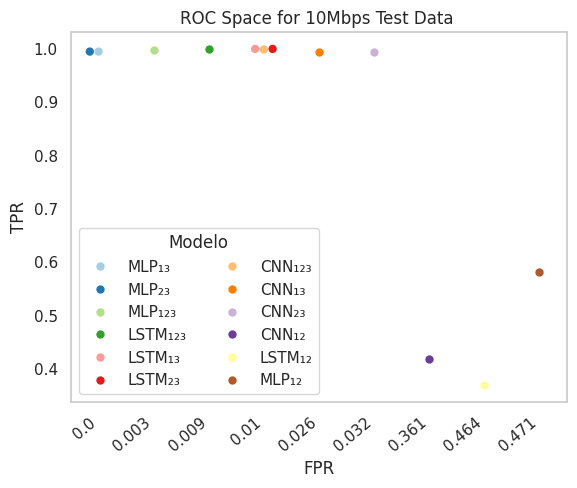
\includegraphics[draft=false, width=\textwidth]{./figs/ROC-Space-Test-Data-10Mbps.png} 
				\caption{Image F}
				\label{fig:1c}
			\end{subfigure}%
			~%Ten que ter uma linha depois do ~
			
			\begin{subfigure}[t]{0.33\textwidth}
				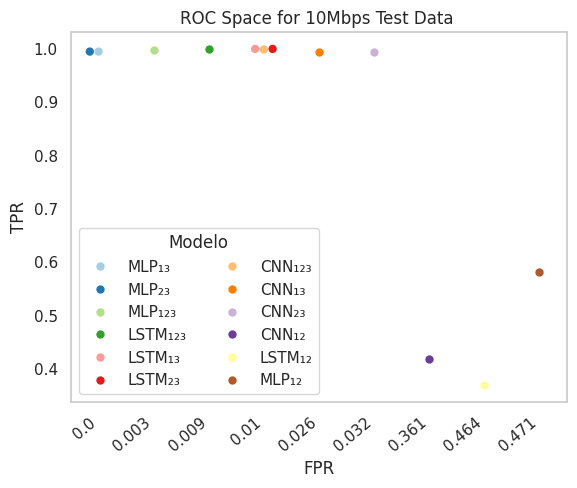
\includegraphics[draft=false, width=\textwidth]{./figs/ROC-Space-Test-Data-10Mbps.png} 
				\caption{Image G}
				\label{fig:1a}
			\end{subfigure}%
			~
			\begin{subfigure}[t]{0.33\textwidth}
				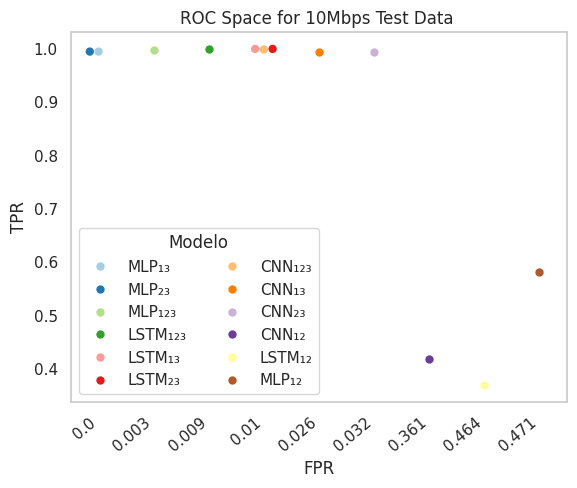
\includegraphics[draft=false, width=\textwidth]{./figs/ROC-Space-Test-Data-10Mbps.png} 
				\caption{Image H}
				\label{fig:2a}
			\end{subfigure}%
			~
			%\medskip % create some vertical separation
			\begin{subfigure}[t]{0.33\textwidth}
				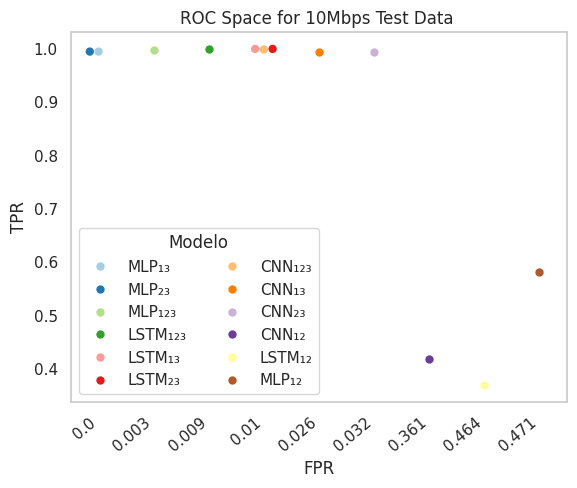
\includegraphics[draft=false, width=\textwidth]{./figs/ROC-Space-Test-Data-10Mbps.png} 
				\caption{Image I}
				\label{fig:1c}
			\end{subfigure}%		
			~
			%}
		\hfill
		\caption{Image Collection 2\hspace{10cm}}
		\label{fig:2}
		%}
\end{minipage}

\end{figure}





\begin{center}

\begin{figure}
	\centering
	\begin{subfigure}[b]{0.45\textwidth}
		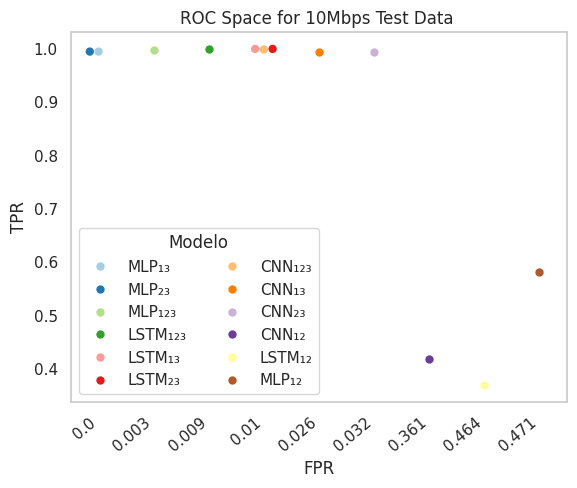
\includegraphics[width=0.3\textwidth]{./figs/ROC-Space-Test-Data-10Mbps.png}		
		\caption{Lorem ipsum}
	    \quad
	 	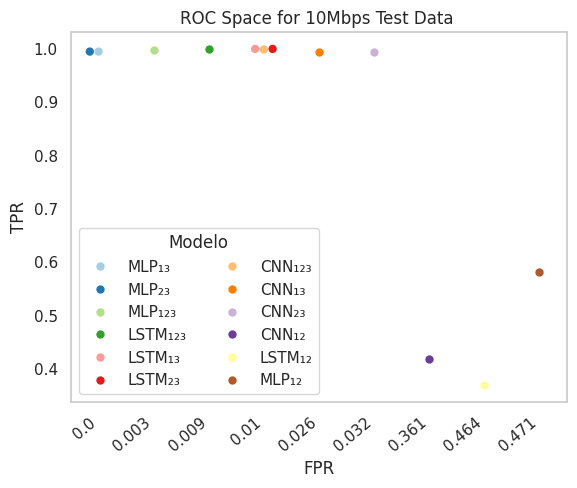
\includegraphics[width=0.3\textwidth]{./figs/ROC-Space-Test-Data-10Mbps.png}
		\caption{Lorem ipsum}
        \quad
		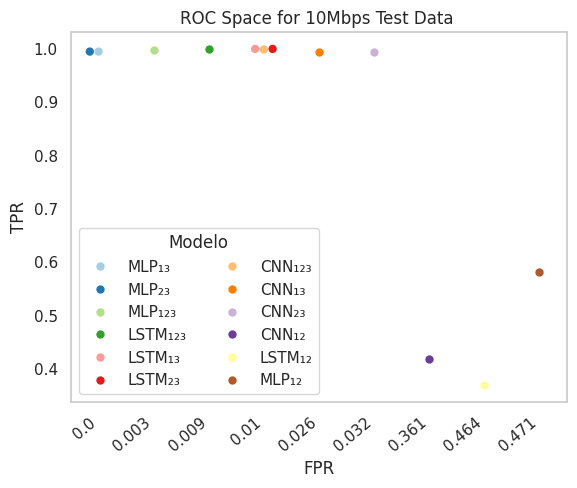
\includegraphics[width=0.3\textwidth]{./figs/ROC-Space-Test-Data-10Mbps.png}
		\caption{Lorem ipsum}
        
		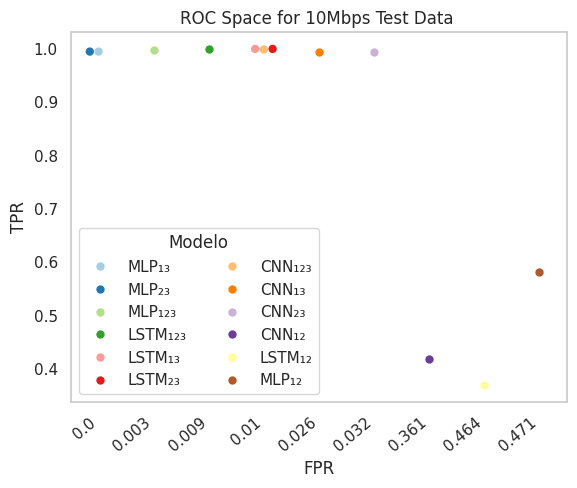
\includegraphics[width=0.3\textwidth]{./figs/ROC-Space-Test-Data-10Mbps.png}
		\caption{Lorem ipsum}
		\quad
		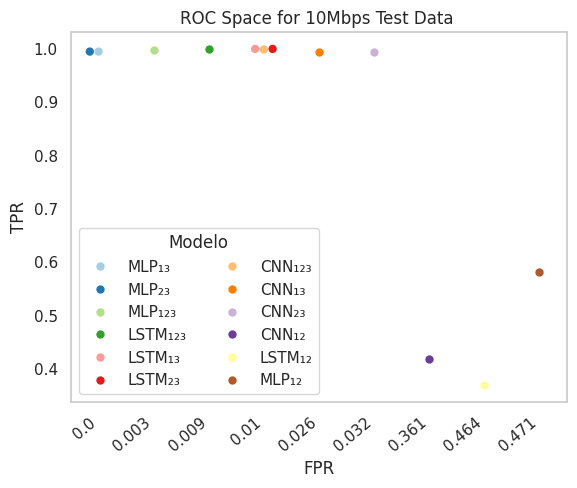
\includegraphics[width=0.3\textwidth]{./figs/ROC-Space-Test-Data-10Mbps.png}
		\caption{Lorem ipsum}
		
		\caption{10Mbps}
	
		\end{subfigure}

	\begin{subfigure}[b]{0.45\textwidth}
		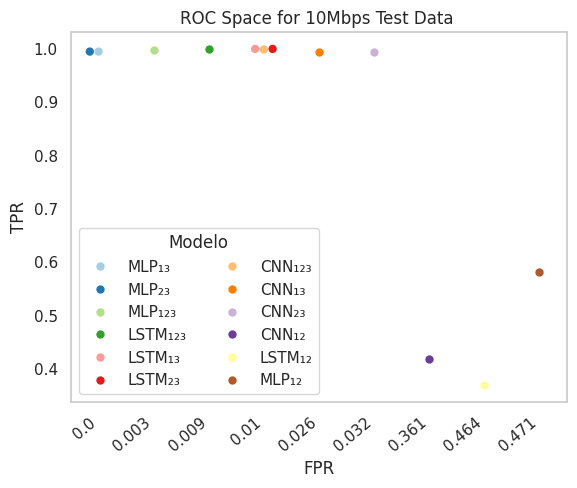
\includegraphics[width=0.3\textwidth]{./figs/ROC-Space-Test-Data-10Mbps.png}		
		\caption{Lorem ipsum}
		\quad
		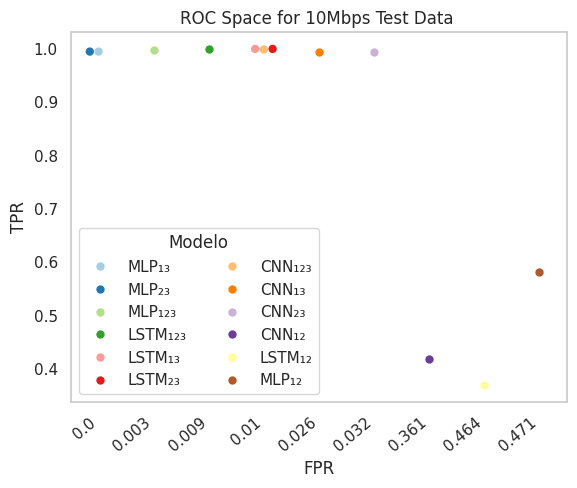
\includegraphics[width=0.3\textwidth]{./figs/ROC-Space-Test-Data-10Mbps.png}
		\caption{Lorem ipsum}
		\quad
		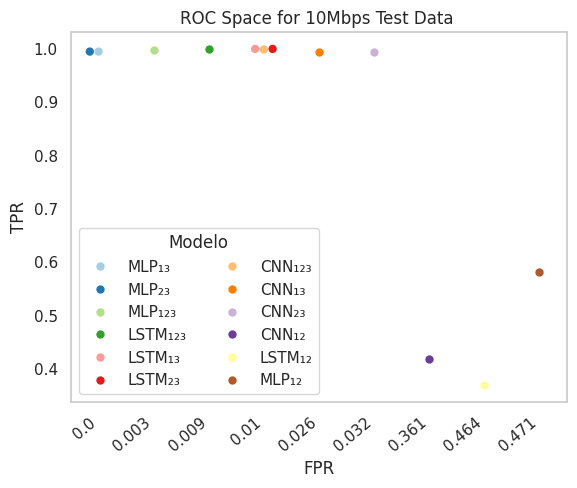
\includegraphics[width=0.3\textwidth]{./figs/ROC-Space-Test-Data-10Mbps.png}
		\caption{Lorem ipsum}
		
		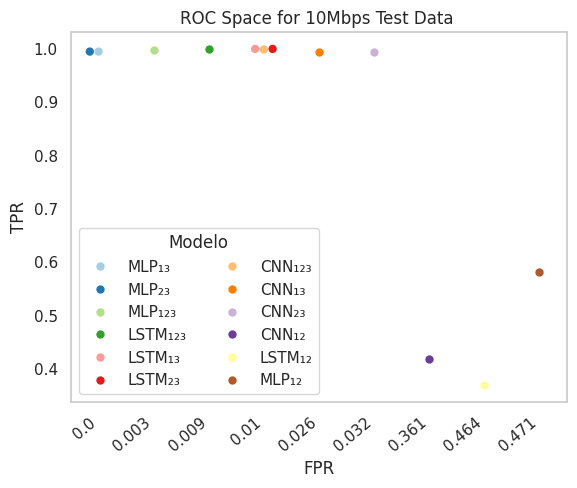
\includegraphics[width=0.3\textwidth]{./figs/ROC-Space-Test-Data-10Mbps.png}
		\caption{Lorem ipsum}
		\quad
		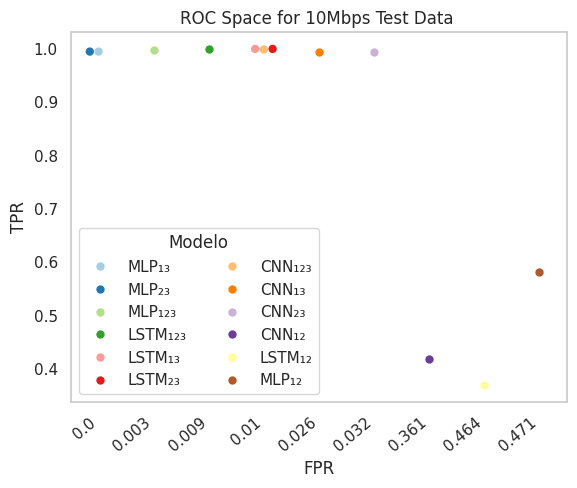
\includegraphics[width=0.3\textwidth]{./figs/ROC-Space-Test-Data-10Mbps.png}
		\caption{Lorem ipsum}
	
	\caption{100Mbps}
	
\end{subfigure}


		\caption{Caption place holder}

\end{figure}

%\end{minipage}

\end{center}




\begin{minipage}{0.45\textwidth}
	\begin{minipage}{0.30\textwidth}
		\centering
		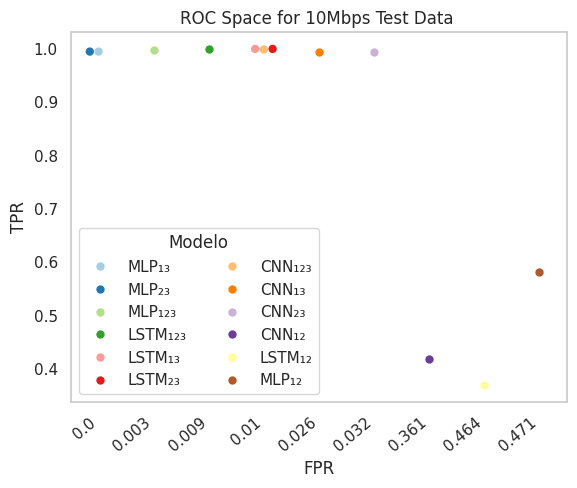
\includegraphics[width=1.0\textwidth]{./figs/ROC-Space-Test-Data-10Mbps.png}
		%\captionof{figure}{ROC space test Data 10Mbps.}
		\label{fig:ROCDesempenhoteste10Mbps}	
	\end{minipage}
	\hfill
	\begin{minipage}{0.30\textwidth}
		\centering
		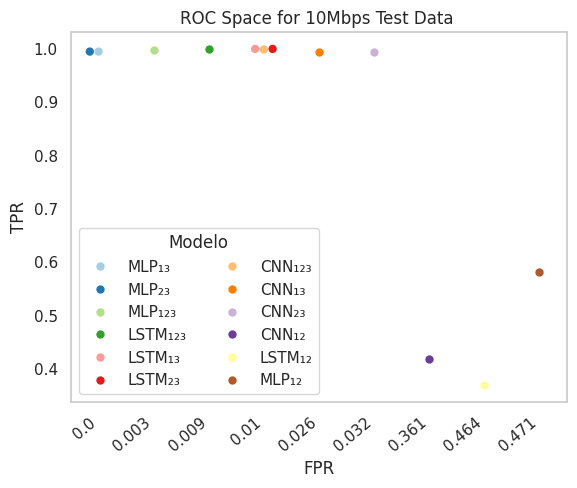
\includegraphics[width=1.0\textwidth]{./figs/ROC-Space-Test-Data-10Mbps.png}
		%\captionof{figure}{ROC space test Data 10Mbps.}
		\label{fig:ROCDesempenhoteste10Mbps}	
	\end{minipage}
	\hfill
	\begin{minipage}{0.30\textwidth}
		\centering
		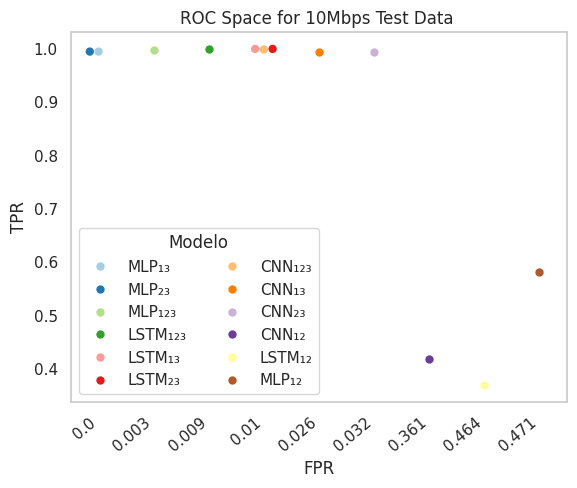
\includegraphics[width=1.0\textwidth]{./figs/ROC-Space-Test-Data-10Mbps.png}
		%\captionof{figure}{ROC space test Data 10Mbps.}
		\label{fig:ROCDesempenhoteste10Mbps}	
	\end{minipage}
	\hfill
	\begin{minipage}{0.30\textwidth}
		\centering
		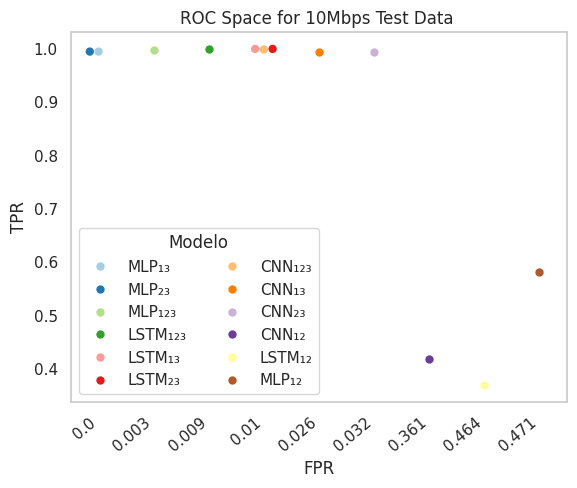
\includegraphics[width=1.0\textwidth]{./figs/ROC-Space-Test-Data-10Mbps.png}
		%\captionof{figure}{ROC space test Data 10Mbps.}
		\label{fig:ROCDesempenhoteste10Mbps}	
	\end{minipage}
	\hfill
	\begin{minipage}{0.30\textwidth}
		\centering
		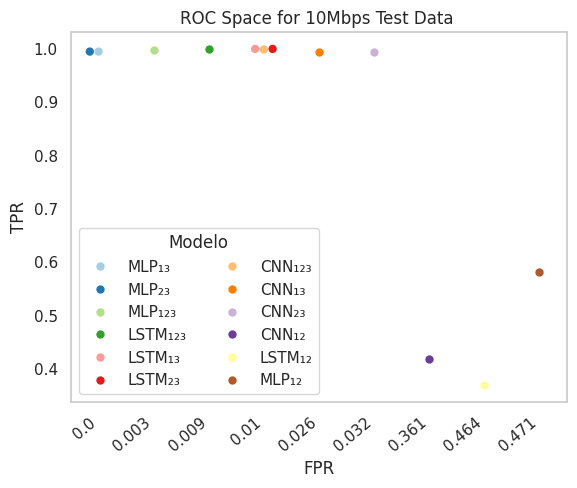
\includegraphics[width=1.0\textwidth]{./figs/ROC-Space-Test-Data-10Mbps.png}
		%\captionof{figure}{ROC space test Data 10Mbps.}
		\label{fig:ROCDesempenhoteste10Mbps}	
	\end{minipage}
	\hfill
	\begin{minipage}{0.30\textwidth}
		\centering
		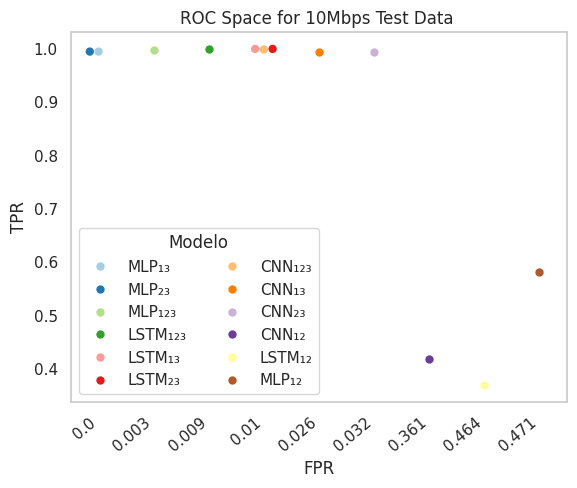
\includegraphics[width=1.0\textwidth]{./figs/ROC-Space-Test-Data-10Mbps.png}
		%\captionof{figure}{ROC space test Data 10Mbps.}
		\label{fig:ROCDesempenhoteste10Mbps}	
	\end{minipage}
	\hfill
	\begin{minipage}{0.30\textwidth}
		\centering
		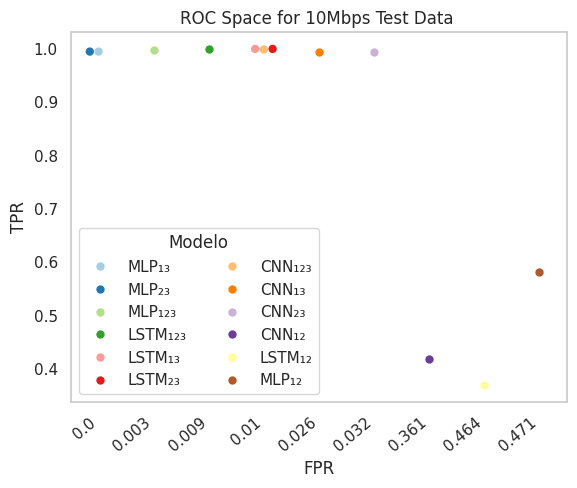
\includegraphics[width=1.0\textwidth]{./figs/ROC-Space-Test-Data-10Mbps.png}
		%\captionof{figure}{ROC space test Data 10Mbps.}
		\label{fig:ROCDesempenhoteste10Mbps}	
	\end{minipage}
	\hfill
	\begin{minipage}{0.30\textwidth}
		\centering
		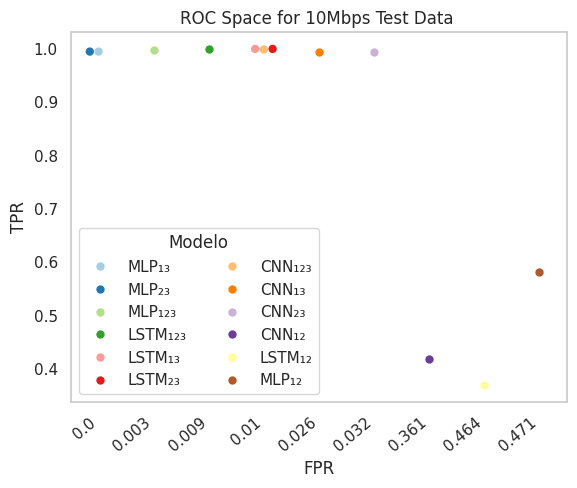
\includegraphics[width=1.0\textwidth]{./figs/ROC-Space-Test-Data-10Mbps.png}
		%\captionof{figure}{ROC space test Data 10Mbps.}
		\label{fig:ROCDesempenhoteste10Mbps}	
	\end{minipage}
	\hfill
	\begin{minipage}{0.30\textwidth}
		\centering
		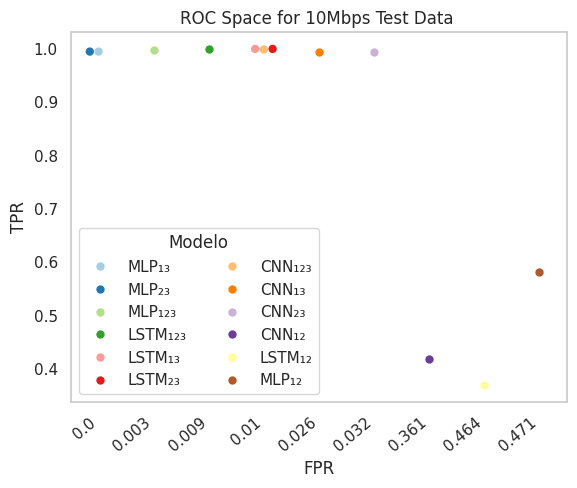
\includegraphics[width=1.0\textwidth]{./figs/ROC-Space-Test-Data-10Mbps.png}
		%\captionof{figure}{ROC space test Data 10Mbps.}
		\label{fig:ROCDesempenhoteste10Mbps}	
	\end{minipage}
	\hfill
	
\end{minipage}










\section{Front matter}

The author names and affiliations could be formatted in two ways:
\begin{enumerate}[(1)]
\item Group the authors per affiliation.
\item Use footnotes to indicate the affiliations.
\end{enumerate}
See the front matter of this document for examples. 
You are recommended to conform your choice to the journal you 
are submitting to.

\section{Bibliography styles}

There are various bibliography styles available. You can select the
style of your choice in the preamble of this document. These styles are
Elsevier styles based on standard styles like Harvard and Vancouver.
Please use Bib\TeX\ to generate your bibliography and include DOIs
whenever available.

Here are two sample references: 
See \citet{Fortunato2010}. Also refer \citet{Fortunato2010,NewmanGirvan2004}.
More citations are here \citep{Fortunato2010,Vehlowetal2013}.

\section{Floats}
{Figures} may be included using the command, \verb+\includegraphics+ in
combination with or without its several options to further control
graphic. \verb+\includegraphics+ is provided by {graphic[s,x].sty}
which is part of any standard \LaTeX{} distribution.
{graphicx.sty} is loaded by default. \LaTeX{} accepts figures in
the postscript format while pdf\LaTeX{} accepts {*.pdf},
{*.mps} (metapost), {*.jpg} and {*.png} formats. 
pdf\LaTeX{} does not accept graphic files in the postscript format. 

\begin{figure}
	\centering
	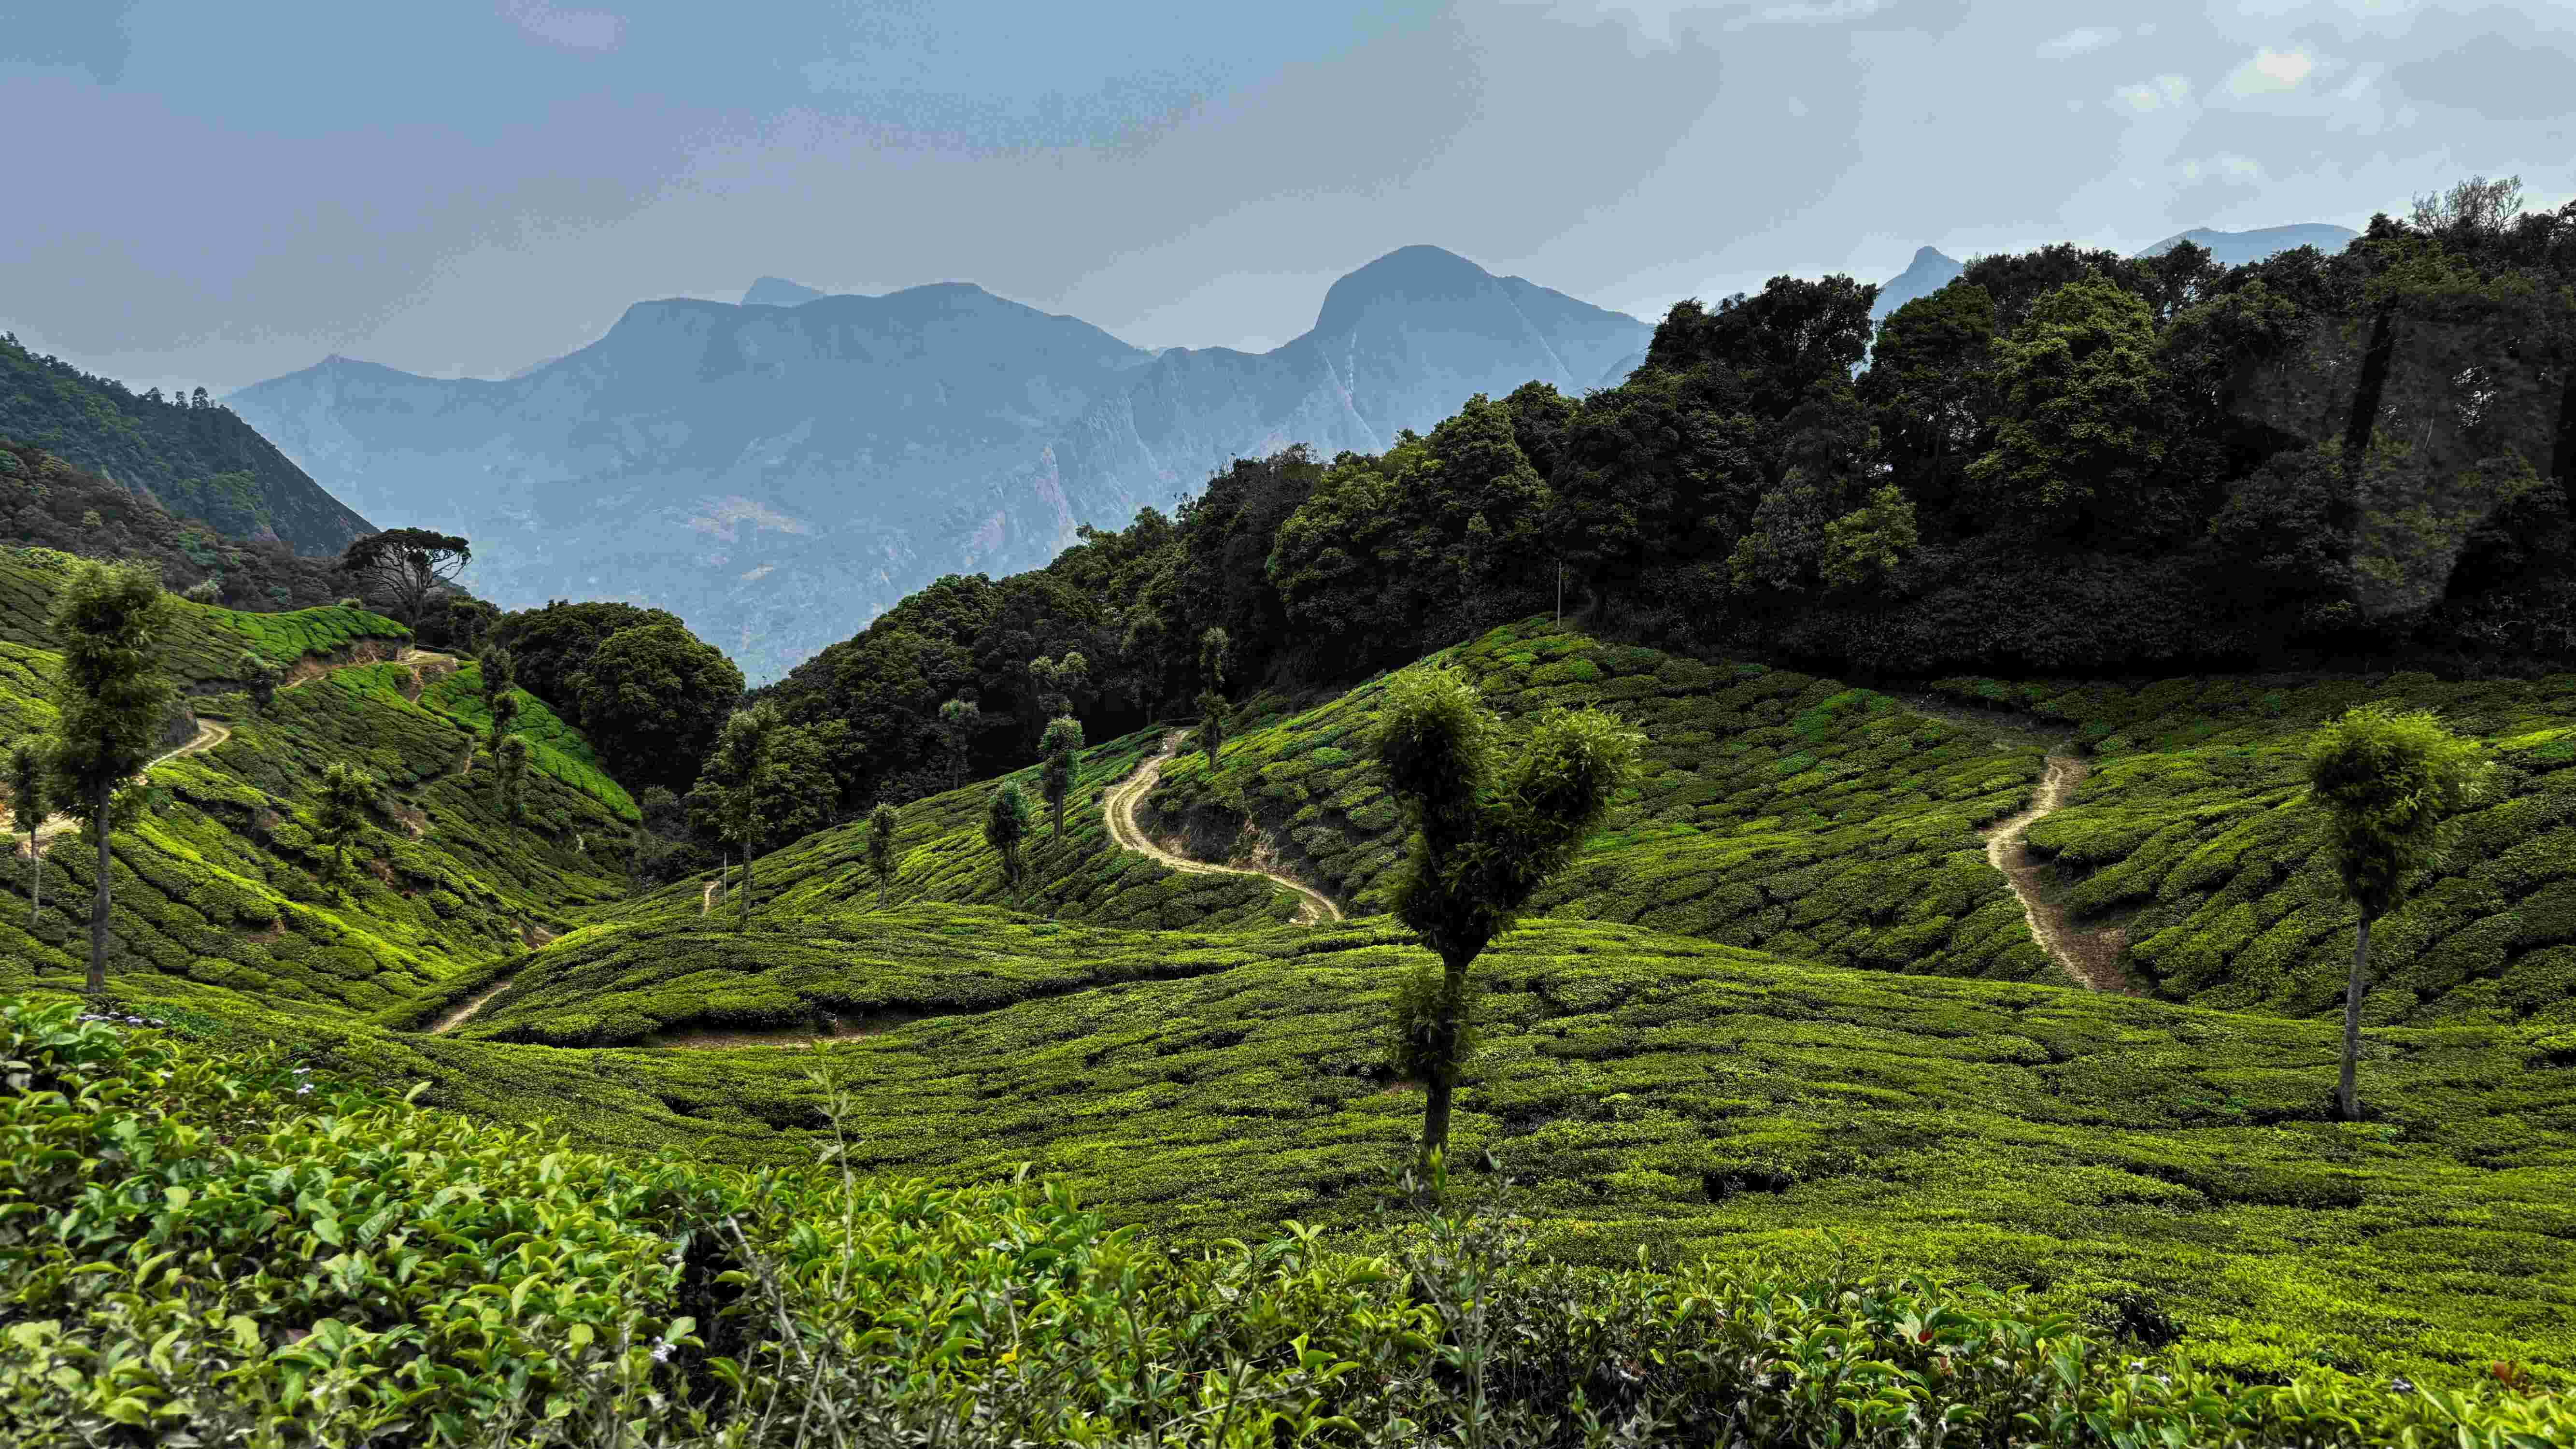
\includegraphics[width=.9\textwidth]{figs/cas-munnar-2024.jpg}
	\caption{The beauty of Munnar, Kerala. (See also Table \protect\ref{tbl1}).}
	\label{FIG:1}
\end{figure}


The \verb+table+ environment is handy for marking up tabular
material. If users want to use {multirow.sty},
{array.sty}, etc., to fine control/enhance the tables, they
are welcome to load any package of their choice and
{cas-sc.cls} will work in combination with all loaded
packages.

\begin{table}[width=.9\linewidth,cols=4,pos=h]
\caption{This is a test caption. This is a test caption. This is a test
caption. This is a test caption.}\label{tbl1}
\begin{tabular*}{\tblwidth}{@{} LLLL@{} }
\toprule
Col 1 & Col 2 & Col 3 & Col4\\
\midrule
12345 & 12345 & 123 & 12345 \\
12345 & 12345 & 123 & 12345 \\
12345 & 12345 & 123 & 12345 \\
12345 & 12345 & 123 & 12345 \\
12345 & 12345 & 123 & 12345 \\
\bottomrule
\end{tabular*}
\end{table}

\section[Theorem and ...]{Theorem and theorem like environments}

{cas-sc.cls} provides a few shortcuts to format theorems and
theorem-like environments with ease. In all commands the options that
are used with the \verb+\newtheorem+ command will work exactly in the same
manner. {cas-sc.cls} provides three commands to format theorem or
theorem-like environments: 

\begin{verbatim}
 \newtheorem{theorem}{Theorem}
 \newtheorem{lemma}[theorem]{Lemma}
 \newdefinition{rmk}{Remark}
 \newproof{pf}{Proof}
 \newproof{pot}{Proof of Theorem \ref{thm2}}
\end{verbatim}


The \verb+\newtheorem+ command formats a
theorem in \LaTeX's default style with italicized font, bold font
for theorem heading and theorem number at the right hand side of the
theorem heading.  It also optionally accepts an argument which
will be printed as an extra heading in parentheses. 

\begin{verbatim}
  \begin{theorem} 
   For system (8), consensus can be achieved with 
   $\|T_{\omega z}$ ...
     \begin{eqnarray}\label{10}
     ....
     \end{eqnarray}
  \end{theorem}
\end{verbatim}  

\newtheorem{theorem}{Theorem}

\begin{theorem}
For system (8), consensus can be achieved with 
$\|T_{\omega z}$ ...
\begin{eqnarray}\label{10}
....
\end{eqnarray}
\end{theorem}

The \verb+\newdefinition+ command is the same in
all respects as its \verb+\newtheorem+ counterpart except that
the font shape is roman instead of italic.  Both
\verb+\newdefinition+ and \verb+\newtheorem+ commands
automatically define counters for the environments defined.

The \verb+\newproof+ command defines proof environments with
upright font shape.  No counters are defined. 


\section[Enumerated ...]{Enumerated and Itemized Lists}
{cas-sc.cls} provides an extended list processing macros
which makes the usage a bit more user friendly than the default
\LaTeX{} list macros.   With an optional argument to the
\verb+\begin{enumerate}+ command, you can change the list counter
type and its attributes.

\begin{verbatim}
 \begin{enumerate}[1.]
 \item The enumerate environment starts with an optional
   argument `1.', so that the item counter will be suffixed
   by a period.
 \item You can use `a)' for alphabetical counter and '(i)' for
   roman counter.
  \begin{enumerate}[a)]
    \item Another level of list with alphabetical counter.
    \item One more item before we start another.
    \item One more item before we start another.
    \item One more item before we start another.
    \item One more item before we start another.
\end{verbatim}

Further, the enhanced list environment allows one to prefix a
string like `step' to all the item numbers.  

%\pagebreak
\begin{verbatim}
 \begin{enumerate}[Step 1.]
  \item This is the first step of the example list.
  \item Obviously this is the second step.
  \item The final step to wind up this example.
 \end{enumerate}
\end{verbatim}

\section{Cross-references}
In electronic publications, articles may be internally
hyperlinked. Hyperlinks are generated from proper
cross-references in the article.  For example, the words
\textcolor{black!80}{Fig.~1} will never be more than simple text,
whereas the proper cross-reference \verb+\ref{tiger}+ may be
turned into a hyperlink to the figure itself:
\textcolor{blue}{Fig.~1}.  In the same way,
the words \textcolor{blue}{Ref.~[1]} will fail to turn into a
hyperlink; the proper cross-reference is \verb+\cite{Knuth96}+.
Cross-referencing is possible in \LaTeX{} for sections,
subsections, formulae, figures, tables, and literature
references.

\section{Bibliography}

Two bibliographic style files (\verb+*.bst+) are provided ---
{model1-num-names.bst} and {model2-names.bst} --- the first one can be
used for the numbered scheme. This can also be used for the numbered
with new options of {natbib.sty}. The second one is for the author year
scheme. When  you use model2-names.bst, the citation commands will be
like \verb+\citep+,  \verb+\citet+, \verb+\citealt+ etc. However when
you use model1-num-names.bst, you may use only \verb+\cite+ command.

\verb+thebibliography+ environment.  Each reference is a
\verb+\bibitem+ and each \verb+\bibitem+ is identified by a label,
by which it can be cited in the text:

\noindent In connection with cross-referencing and
possible future hyperlinking it is not a good idea to collect
more that one literature item in one \verb+\bibitem+.  The
so-called Harvard or author-year style of referencing is enabled
by the \LaTeX{} package {natbib}. With this package the
literature can be cited as follows:


\begin{enumerate}[\textbullet]
\item Parenthetical: \verb+\citep{WB96}+ produces (Wettig \& Brown, 1996).
\item Textual: \verb+\citet{ESG96}+ produces Elson et al. (1996).
\item An affix and part of a reference:
\verb+\citep[e.g.][Ch. 2]{Gea97}+ produces (e.g. Governato et
al., 1997, Ch. 2).
\end{enumerate}

In the numbered scheme of citation, \verb+\cite{<label>}+ is used,
since \verb+\citep+ or \verb+\citet+ has no relevance in the numbered
scheme.  {natbib} package is loaded by {cas-sc} with
\verb+numbers+ as default option.  You can change this to author-year
or harvard scheme by adding option \verb+authoryear+ in the class
loading command.  If you want to use more options of the {natbib}
package, you can do so with the \verb+\biboptions+ command.  For
details of various options of the {natbib} package, please take a
look at the {natbib} documentation, which is part of any standard
\LaTeX{} installation.

\appendix
\section{My Appendix}
Appendix sections are coded under \verb+\appendix+.

\verb+\printcredits+ command is used after appendix sections to list 
author credit taxonomy contribution roles tagged using \verb+\credit+ 
in frontmatter.

\printcredits

%% Loading bibliography style file
%\bibliographystyle{model1-num-names}
\bibliographystyle{cas-model2-names}

% Loading bibliography database
\bibliography{cas-refs}


%\vskip3pt

\bio{}
Author biography without author photo.
Author biography. Author biography. Author biography.
Author biography. Author biography. Author biography.
Author biography. Author biography. Author biography.
Author biography. Author biography. Author biography.
Author biography. Author biography. Author biography.
Author biography. Author biography. Author biography.
Author biography. Author biography. Author biography.
Author biography. Author biography. Author biography.
Author biography. Author biography. Author biography.
\endbio

\bio{figs/cas-pic1}
Author biography with author photo.
Author biography. Author biography. Author biography.
Author biography. Author biography. Author biography.
Author biography. Author biography. Author biography.
Author biography. Author biography. Author biography.
Author biography. Author biography. Author biography.
Author biography. Author biography. Author biography.
Author biography. Author biography. Author biography.
Author biography. Author biography. Author biography.
Author biography. Author biography. Author biography.
\endbio

\vskip3pc

\bio{figs/cas-pic1}
Author biography with author photo.
Author biography. Author biography. Author biography.
Author biography. Author biography. Author biography.
Author biography. Author biography. Author biography.
Author biography. Author biography. Author biography.
\endbio


\end{document}

